\documentclass[a4paper]{article}
\usepackage[margin=1in]{geometry}
\usepackage[utf8]{inputenc}
\usepackage[spanish]{babel}
\usepackage{amsmath, amsthm, amsfonts, amssymb, mathrsfs}
\usepackage{hyperref,fancyhdr}
\usepackage{booktabs}% fancy tables
\usepackage{tocloft}% agregar tabla de preguntas 
%\usepackage{multicol}
\usepackage{graphicx}
\usepackage{capt-of}
\setlength{\columnsep}{1cm}
\IfFileExists{lmodern.sty}{\usepackage{lmodern}}{}
\usepackage[T1]{fontenc}
\IfFileExists{lmodern.sty}{\usepackage{lmodern}}{}
\usepackage[T1]{fontenc}
\usepackage[utf8]{inputenc}
\usepackage{tikz}
\usepackage{gnuplottex}
\usetikzlibrary{decorations.pathreplacing}
\author{Carlos Rodrigo Sanabria Flores}
\hypersetup{
    pdftitle={Praticas PCTR},
    pdfsubject={PCTR},
    pdfauthor={Carlos Rodrigo Sanbria},
    pdfkeywords={PCTR, JAVA, TEX}
}
\title{Rendimiento CPU}
\begin{document}
\pagestyle{fancy}
\fancyhf{}
\renewcommand{\headrulewidth}{0mm}
\cfoot{\thepage}
\setlength{\parskip}{2em}
\newenvironment{Table}
    {\par\bigskip\noindent\minipage{\columnwidth}\centering}
    {\endminipage\par\bigskip}
\newcommand{\question}[1] % This is what you will use to create a new question
{%\refstepcounter{questions} % Increases the questions counter, this can be referenced anywhere with \thequestions
\par\noindent % Creates a new unindented paragraph
\phantomsection % Needed for hyperref compatibility with the \addcontensline command
%\addcontentsline{faq}{questions}{#1} % Adds the question to the list of questions
{\textbf{#1}}%\todo[inline, color=green!40] % Uses the todonotes package to create a fancy box to put the question
\vspace{1em} % White space after the question before the start of the answer
}
\maketitle
\begin{abstract}
    \centering
    Picos de uso de cpu respecto al tiempo de ejecucion en el escalado de un vector paralelamente de $10^8$ elementos.
\end{abstract}
\begin{figure}[!htb]
    \centering
    \includegraphics[scale=.5]{vectordimensioncpu.eps}
    \caption{Matriz - Vector}
    \label{fig:digraph}
\end{figure}
\begin{figure}[!htb]
    \centering
    \includegraphics[scale=.5]{vectordimensiontiempo.eps}
    \caption{Matriz - Vector}
    \label{fig:digraph}
\end{figure}
\begin{figure}[!htb]
    \centering
    \includegraphics[scale=.5]{matrizdimensiocpu.eps}
    \caption{Matriz - Matriz}
    \label{fig:digraph}
\end{figure}
\begin{figure}[!htb]
    \centering
    \includegraphics[scale=.5]{matrizdimensiotiempo.eps}
    \caption{Matriz - Matriz}
    \label{fig:digraph}
\end{figure}
\end{document}